% Options for packages loaded elsewhere
\PassOptionsToPackage{unicode}{hyperref}
\PassOptionsToPackage{hyphens}{url}
\PassOptionsToPackage{dvipsnames,svgnames,x11names}{xcolor}
%
\documentclass[
  letterpaper,
  DIV=11,
  numbers=noendperiod]{scrartcl}

\usepackage{amsmath,amssymb}
\usepackage{lmodern}
\usepackage{iftex}
\ifPDFTeX
  \usepackage[T1]{fontenc}
  \usepackage[utf8]{inputenc}
  \usepackage{textcomp} % provide euro and other symbols
\else % if luatex or xetex
  \usepackage{unicode-math}
  \defaultfontfeatures{Scale=MatchLowercase}
  \defaultfontfeatures[\rmfamily]{Ligatures=TeX,Scale=1}
\fi
% Use upquote if available, for straight quotes in verbatim environments
\IfFileExists{upquote.sty}{\usepackage{upquote}}{}
\IfFileExists{microtype.sty}{% use microtype if available
  \usepackage[]{microtype}
  \UseMicrotypeSet[protrusion]{basicmath} % disable protrusion for tt fonts
}{}
\makeatletter
\@ifundefined{KOMAClassName}{% if non-KOMA class
  \IfFileExists{parskip.sty}{%
    \usepackage{parskip}
  }{% else
    \setlength{\parindent}{0pt}
    \setlength{\parskip}{6pt plus 2pt minus 1pt}}
}{% if KOMA class
  \KOMAoptions{parskip=half}}
\makeatother
\usepackage{xcolor}
\setlength{\emergencystretch}{3em} % prevent overfull lines
\setcounter{secnumdepth}{5}
% Make \paragraph and \subparagraph free-standing
\ifx\paragraph\undefined\else
  \let\oldparagraph\paragraph
  \renewcommand{\paragraph}[1]{\oldparagraph{#1}\mbox{}}
\fi
\ifx\subparagraph\undefined\else
  \let\oldsubparagraph\subparagraph
  \renewcommand{\subparagraph}[1]{\oldsubparagraph{#1}\mbox{}}
\fi

\usepackage{color}
\usepackage{fancyvrb}
\newcommand{\VerbBar}{|}
\newcommand{\VERB}{\Verb[commandchars=\\\{\}]}
\DefineVerbatimEnvironment{Highlighting}{Verbatim}{commandchars=\\\{\}}
% Add ',fontsize=\small' for more characters per line
\usepackage{framed}
\definecolor{shadecolor}{RGB}{241,243,245}
\newenvironment{Shaded}{\begin{snugshade}}{\end{snugshade}}
\newcommand{\AlertTok}[1]{\textcolor[rgb]{0.68,0.00,0.00}{#1}}
\newcommand{\AnnotationTok}[1]{\textcolor[rgb]{0.37,0.37,0.37}{#1}}
\newcommand{\AttributeTok}[1]{\textcolor[rgb]{0.40,0.45,0.13}{#1}}
\newcommand{\BaseNTok}[1]{\textcolor[rgb]{0.68,0.00,0.00}{#1}}
\newcommand{\BuiltInTok}[1]{\textcolor[rgb]{0.00,0.23,0.31}{#1}}
\newcommand{\CharTok}[1]{\textcolor[rgb]{0.13,0.47,0.30}{#1}}
\newcommand{\CommentTok}[1]{\textcolor[rgb]{0.37,0.37,0.37}{#1}}
\newcommand{\CommentVarTok}[1]{\textcolor[rgb]{0.37,0.37,0.37}{\textit{#1}}}
\newcommand{\ConstantTok}[1]{\textcolor[rgb]{0.56,0.35,0.01}{#1}}
\newcommand{\ControlFlowTok}[1]{\textcolor[rgb]{0.00,0.23,0.31}{#1}}
\newcommand{\DataTypeTok}[1]{\textcolor[rgb]{0.68,0.00,0.00}{#1}}
\newcommand{\DecValTok}[1]{\textcolor[rgb]{0.68,0.00,0.00}{#1}}
\newcommand{\DocumentationTok}[1]{\textcolor[rgb]{0.37,0.37,0.37}{\textit{#1}}}
\newcommand{\ErrorTok}[1]{\textcolor[rgb]{0.68,0.00,0.00}{#1}}
\newcommand{\ExtensionTok}[1]{\textcolor[rgb]{0.00,0.23,0.31}{#1}}
\newcommand{\FloatTok}[1]{\textcolor[rgb]{0.68,0.00,0.00}{#1}}
\newcommand{\FunctionTok}[1]{\textcolor[rgb]{0.28,0.35,0.67}{#1}}
\newcommand{\ImportTok}[1]{\textcolor[rgb]{0.00,0.46,0.62}{#1}}
\newcommand{\InformationTok}[1]{\textcolor[rgb]{0.37,0.37,0.37}{#1}}
\newcommand{\KeywordTok}[1]{\textcolor[rgb]{0.00,0.23,0.31}{#1}}
\newcommand{\NormalTok}[1]{\textcolor[rgb]{0.00,0.23,0.31}{#1}}
\newcommand{\OperatorTok}[1]{\textcolor[rgb]{0.37,0.37,0.37}{#1}}
\newcommand{\OtherTok}[1]{\textcolor[rgb]{0.00,0.23,0.31}{#1}}
\newcommand{\PreprocessorTok}[1]{\textcolor[rgb]{0.68,0.00,0.00}{#1}}
\newcommand{\RegionMarkerTok}[1]{\textcolor[rgb]{0.00,0.23,0.31}{#1}}
\newcommand{\SpecialCharTok}[1]{\textcolor[rgb]{0.37,0.37,0.37}{#1}}
\newcommand{\SpecialStringTok}[1]{\textcolor[rgb]{0.13,0.47,0.30}{#1}}
\newcommand{\StringTok}[1]{\textcolor[rgb]{0.13,0.47,0.30}{#1}}
\newcommand{\VariableTok}[1]{\textcolor[rgb]{0.07,0.07,0.07}{#1}}
\newcommand{\VerbatimStringTok}[1]{\textcolor[rgb]{0.13,0.47,0.30}{#1}}
\newcommand{\WarningTok}[1]{\textcolor[rgb]{0.37,0.37,0.37}{\textit{#1}}}

\providecommand{\tightlist}{%
  \setlength{\itemsep}{0pt}\setlength{\parskip}{0pt}}\usepackage{longtable,booktabs,array}
\usepackage{calc} % for calculating minipage widths
% Correct order of tables after \paragraph or \subparagraph
\usepackage{etoolbox}
\makeatletter
\patchcmd\longtable{\par}{\if@noskipsec\mbox{}\fi\par}{}{}
\makeatother
% Allow footnotes in longtable head/foot
\IfFileExists{footnotehyper.sty}{\usepackage{footnotehyper}}{\usepackage{footnote}}
\makesavenoteenv{longtable}
\usepackage{graphicx}
\makeatletter
\def\maxwidth{\ifdim\Gin@nat@width>\linewidth\linewidth\else\Gin@nat@width\fi}
\def\maxheight{\ifdim\Gin@nat@height>\textheight\textheight\else\Gin@nat@height\fi}
\makeatother
% Scale images if necessary, so that they will not overflow the page
% margins by default, and it is still possible to overwrite the defaults
% using explicit options in \includegraphics[width, height, ...]{}
\setkeys{Gin}{width=\maxwidth,height=\maxheight,keepaspectratio}
% Set default figure placement to htbp
\makeatletter
\def\fps@figure{htbp}
\makeatother

\KOMAoption{captions}{tableheading}
\makeatletter
\@ifpackageloaded{tcolorbox}{}{\usepackage[many]{tcolorbox}}
\@ifpackageloaded{fontawesome5}{}{\usepackage{fontawesome5}}
\definecolor{quarto-callout-color}{HTML}{909090}
\definecolor{quarto-callout-note-color}{HTML}{0758E5}
\definecolor{quarto-callout-important-color}{HTML}{CC1914}
\definecolor{quarto-callout-warning-color}{HTML}{EB9113}
\definecolor{quarto-callout-tip-color}{HTML}{00A047}
\definecolor{quarto-callout-caution-color}{HTML}{FC5300}
\definecolor{quarto-callout-color-frame}{HTML}{acacac}
\definecolor{quarto-callout-note-color-frame}{HTML}{4582ec}
\definecolor{quarto-callout-important-color-frame}{HTML}{d9534f}
\definecolor{quarto-callout-warning-color-frame}{HTML}{f0ad4e}
\definecolor{quarto-callout-tip-color-frame}{HTML}{02b875}
\definecolor{quarto-callout-caution-color-frame}{HTML}{fd7e14}
\makeatother
\makeatletter
\makeatother
\makeatletter
\makeatother
\makeatletter
\@ifpackageloaded{caption}{}{\usepackage{caption}}
\AtBeginDocument{%
\ifdefined\contentsname
  \renewcommand*\contentsname{Table of contents}
\else
  \newcommand\contentsname{Table of contents}
\fi
\ifdefined\listfigurename
  \renewcommand*\listfigurename{List of Figures}
\else
  \newcommand\listfigurename{List of Figures}
\fi
\ifdefined\listtablename
  \renewcommand*\listtablename{List of Tables}
\else
  \newcommand\listtablename{List of Tables}
\fi
\ifdefined\figurename
  \renewcommand*\figurename{Figure}
\else
  \newcommand\figurename{Figure}
\fi
\ifdefined\tablename
  \renewcommand*\tablename{Table}
\else
  \newcommand\tablename{Table}
\fi
}
\@ifpackageloaded{float}{}{\usepackage{float}}
\floatstyle{ruled}
\@ifundefined{c@chapter}{\newfloat{codelisting}{h}{lop}}{\newfloat{codelisting}{h}{lop}[chapter]}
\floatname{codelisting}{Listing}
\newcommand*\listoflistings{\listof{codelisting}{List of Listings}}
\makeatother
\makeatletter
\@ifpackageloaded{caption}{}{\usepackage{caption}}
\@ifpackageloaded{subcaption}{}{\usepackage{subcaption}}
\makeatother
\makeatletter
\@ifpackageloaded{tcolorbox}{}{\usepackage[many]{tcolorbox}}
\makeatother
\makeatletter
\@ifundefined{shadecolor}{\definecolor{shadecolor}{rgb}{.97, .97, .97}}
\makeatother
\makeatletter
\makeatother
\ifLuaTeX
  \usepackage{selnolig}  % disable illegal ligatures
\fi
\IfFileExists{bookmark.sty}{\usepackage{bookmark}}{\usepackage{hyperref}}
\IfFileExists{xurl.sty}{\usepackage{xurl}}{} % add URL line breaks if available
\urlstyle{same} % disable monospaced font for URLs
\hypersetup{
  pdftitle={A Quick Introduction to R},
  pdfauthor={Andy Grogan-Kaylor},
  colorlinks=true,
  linkcolor={blue},
  filecolor={Maroon},
  citecolor={Blue},
  urlcolor={Blue},
  pdfcreator={LaTeX via pandoc}}

\title{A Quick Introduction to R}
\author{Andy Grogan-Kaylor}
\date{6/19/23}

\begin{document}
\maketitle
\ifdefined\Shaded\renewenvironment{Shaded}{\begin{tcolorbox}[interior hidden, boxrule=0pt, borderline west={3pt}{0pt}{shadecolor}, frame hidden, enhanced, sharp corners, breakable]}{\end{tcolorbox}}\fi

\hypertarget{why-use-r}{%
\section{Why Use R?}\label{why-use-r}}

R has a reputation for being difficult to learn, and a lot of that
reputation is deserved. However, it is possible to teach R in an
accessible way, and \textbf{a little bit of R can take you a long way}.

\href{https://www.r-project.org/}{R} is open source, and therefore free,
statistical software that is particularly good at obtaining, analyzing
and visualizing data.

R Commands are stored in a \emph{script} or \emph{code} file that
usually ends in .R, e.g.~\texttt{myscript.R}. The command file is
distinct from your actual data, stored in an .RData file,
e.g.~\texttt{mydata.RData}.

A great deal of data analysis and visualization involves the same core
set of steps.

Given the fact that we often want to apply the same core set of tasks to
new questions and new data, there are ways to overcome the steep
learning curve and learn a replicable set of commands that can be
applied to problem after problem. \textbf{The same 5 to 10 lines of R
code can often be tweaked over and over again for multiple projects.}

\[\text{have a question} \rightarrow \text{get data} \rightarrow \text{process and clean data} \rightarrow\]
\[\text{visualize data} \rightarrow \text{analyze data} \rightarrow \text{make conclusions}\]

\hypertarget{get-r}{%
\section{Get R}\label{get-r}}

\href{https://www.r-project.org/}{R} is available at
\url{https://www.r-project.org/}. R is a lot easier to run if you run it
from RStudio, \url{http://www.rstudio.com}.

\hypertarget{get-data}{%
\section{Get Data}\label{get-data}}

Data often comes from other types of data files like SPSS, Stata, or
Excel. Especially in beginning R programming, getting the data into R
can be the most complicated part of your program.

\begin{Shaded}
\begin{Highlighting}[]
\FunctionTok{load}\NormalTok{(}\StringTok{"the/path/to/mydata.Rdata"}\NormalTok{) }\CommentTok{\# data in R format}

\FunctionTok{library}\NormalTok{(haven) }\CommentTok{\# library for importing data }
\NormalTok{mydata }\OtherTok{\textless{}{-}} \FunctionTok{read\_sav}\NormalTok{(}\StringTok{"the/path/to/mySPSSfile.sav"}\NormalTok{) }\CommentTok{\# SPSS}
\NormalTok{mydata }\OtherTok{\textless{}{-}} \FunctionTok{read\_dta}\NormalTok{(}\StringTok{"the/path/to/myStatafile.dta"}\NormalTok{) }\CommentTok{\# Stata}

\FunctionTok{library}\NormalTok{(readxl) }\CommentTok{\# library for importing Excel files}
\NormalTok{mydata }\OtherTok{\textless{}{-}} \FunctionTok{read\_excel}\NormalTok{(}\StringTok{"the/path/to/mySpreadsheet.xls"}\NormalTok{)}

\FunctionTok{save}\NormalTok{(mydata, }\AttributeTok{file =} \StringTok{"mydata.RData"}\NormalTok{) }\CommentTok{\# save in R format}
\end{Highlighting}
\end{Shaded}

\hypertarget{process-and-clean-data}{%
\section{Process and Clean Data}\label{process-and-clean-data}}

The \texttt{\$} sign is a kind of ``connector''. \texttt{mydata\$x}
means: ``The variable \texttt{x} in the dataset called
\texttt{mydata}''.

\begin{Shaded}
\begin{Highlighting}[]
\NormalTok{mydata}\SpecialCharTok{$}\NormalTok{x[mydata}\SpecialCharTok{$}\NormalTok{x }\SpecialCharTok{==} \SpecialCharTok{{-}}\DecValTok{9}\NormalTok{] }\OtherTok{\textless{}{-}} \ConstantTok{NA} \CommentTok{\# missing to NA}
\end{Highlighting}
\end{Shaded}

R makes a strong distinction between \emph{continuous} \emph{numeric}
variables that measure scales like mental health or neighborhood safety,
and \emph{categorical} \emph{factor variables} that measure non-ordered
categories like religious identity or gender identity.

Many statistical and graphical procedures are designed to recognize and
work with different variable types. You often \emph{don't} need to use
all of the options.
e.g.~\texttt{mydata\$w\ \textless{}-\ factor(mydata\$z)} will often work
just fine. \textbf{Changing variables from factor to numeric, and vice
versa can sometimes be the simple solution that solves a lot of problems
when you are trying to graph your variables.}

\begin{Shaded}
\begin{Highlighting}[]
\NormalTok{mydata}\SpecialCharTok{$}\NormalTok{w }\OtherTok{\textless{}{-}} \FunctionTok{factor}\NormalTok{(mydata}\SpecialCharTok{$}\NormalTok{z, }\CommentTok{\# original numeric variable}
                   \AttributeTok{levels =} \FunctionTok{c}\NormalTok{(}\DecValTok{0}\NormalTok{, }\DecValTok{1}\NormalTok{, }\DecValTok{2}\NormalTok{), }
                   \AttributeTok{labels =} \FunctionTok{c}\NormalTok{(}\StringTok{"Group A"}\NormalTok{, }\StringTok{"Group B"}\NormalTok{, }\StringTok{"Group C"}\NormalTok{), }
                   \AttributeTok{ordered =} \ConstantTok{TRUE}\NormalTok{) }\CommentTok{\# whether order matters}

\NormalTok{mydata}\SpecialCharTok{$}\NormalTok{z }\OtherTok{\textless{}{-}} \FunctionTok{as.numeric}\NormalTok{(mydata}\SpecialCharTok{$}\NormalTok{w) }\CommentTok{\# factor to numeric}
\end{Highlighting}
\end{Shaded}

\hypertarget{visualize-data}{%
\section{Visualize Data}\label{visualize-data}}

\hypertarget{histogram}{%
\subsection{Histogram}\label{histogram}}

\begin{Shaded}
\begin{Highlighting}[]
\FunctionTok{hist}\NormalTok{(mydata}\SpecialCharTok{$}\NormalTok{x, }\CommentTok{\# what I\textquotesingle{}m graphing}
     \AttributeTok{main =} \StringTok{"your title goes here"}\NormalTok{, }\CommentTok{\# title}
     \AttributeTok{xlab =} \StringTok{"income"}\NormalTok{, }\CommentTok{\# label for x axis}
     \AttributeTok{col =} \StringTok{"blue"}\NormalTok{) }\CommentTok{\# color}
\end{Highlighting}
\end{Shaded}

\begin{figure}[H]

{\centering 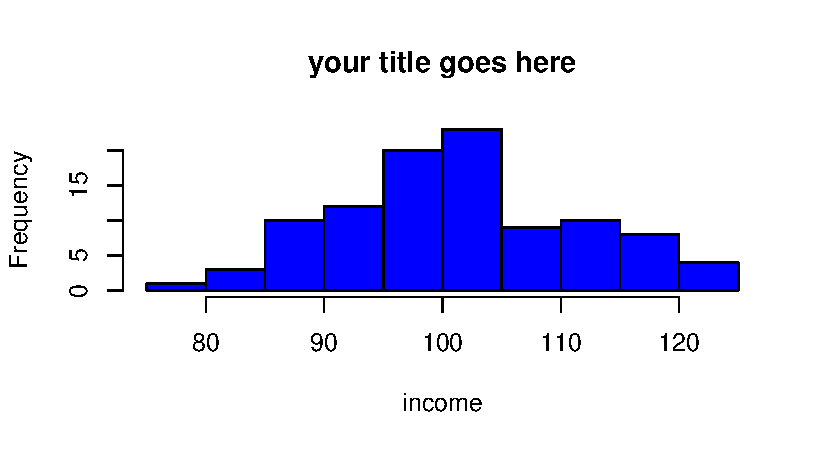
\includegraphics{quick-intro-R_files/figure-pdf/unnamed-chunk-6-1.pdf}

}

\end{figure}

\begin{tcolorbox}[enhanced jigsaw, toptitle=1mm, opacityback=0, colbacktitle=quarto-callout-tip-color!10!white, opacitybacktitle=0.6, arc=.35mm, colframe=quarto-callout-tip-color-frame, coltitle=black, bottomrule=.15mm, leftrule=.75mm, breakable, bottomtitle=1mm, left=2mm, titlerule=0mm, toprule=.15mm, rightrule=.15mm, title=\textcolor{quarto-callout-tip-color}{\faLightbulb}\hspace{0.5em}{Tip}, colback=white]

You often \emph{don't} need to use all of the options.
e.g.~\texttt{hist(mydata\$x)} will work just fine.

\end{tcolorbox}

\hypertarget{barplot}{%
\subsection{Barplot}\label{barplot}}

\begin{Shaded}
\begin{Highlighting}[]
\FunctionTok{barplot}\NormalTok{(}\FunctionTok{table}\NormalTok{(mydata}\SpecialCharTok{$}\NormalTok{z), }\CommentTok{\# what I\textquotesingle{}m graphing}
        \AttributeTok{names.arg =} \FunctionTok{c}\NormalTok{(}\StringTok{"Group A"}\NormalTok{, }\StringTok{"Group B"}\NormalTok{), }\CommentTok{\# names}
        \AttributeTok{main =} \StringTok{"your title goes here"}\NormalTok{, }\CommentTok{\# title}
        \AttributeTok{xlab =} \StringTok{"group"}\NormalTok{, }\CommentTok{\# label for x axis}
        \AttributeTok{col =} \StringTok{"gold"}\NormalTok{) }\CommentTok{\# color}
\end{Highlighting}
\end{Shaded}

\begin{figure}[H]

{\centering 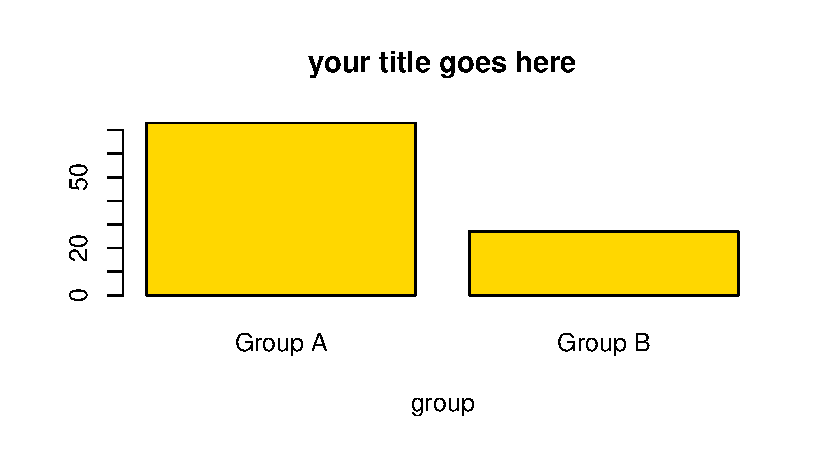
\includegraphics{quick-intro-R_files/figure-pdf/unnamed-chunk-7-1.pdf}

}

\end{figure}

\begin{tcolorbox}[enhanced jigsaw, toptitle=1mm, opacityback=0, colbacktitle=quarto-callout-tip-color!10!white, opacitybacktitle=0.6, arc=.35mm, colframe=quarto-callout-tip-color-frame, coltitle=black, bottomrule=.15mm, leftrule=.75mm, breakable, bottomtitle=1mm, left=2mm, titlerule=0mm, toprule=.15mm, rightrule=.15mm, title=\textcolor{quarto-callout-tip-color}{\faLightbulb}\hspace{0.5em}{Tip}, colback=white]

You often \emph{don't} need to use all of the options.
e.g.~\texttt{barplot(table(mydata\$z))} will work just fine.

\end{tcolorbox}

\hypertarget{scatterplot}{%
\subsection{Scatterplot}\label{scatterplot}}

\begin{Shaded}
\begin{Highlighting}[]
\FunctionTok{plot}\NormalTok{(mydata}\SpecialCharTok{$}\NormalTok{x, mydata}\SpecialCharTok{$}\NormalTok{y, }\CommentTok{\# plot x and y}
     \AttributeTok{main =} \StringTok{"your title goes here"}\NormalTok{, }\CommentTok{\# title}
     \AttributeTok{xlab =} \StringTok{"income"}\NormalTok{, }\CommentTok{\# label for x axis}
     \AttributeTok{ylab =} \StringTok{"mental health"}\NormalTok{, }\CommentTok{\# label for y axis}
     \AttributeTok{pch =} \DecValTok{19}\NormalTok{, }\CommentTok{\# Plot CHaracter, 19 is filled dots}
     \AttributeTok{las =} \DecValTok{2}\NormalTok{, }\CommentTok{\# LAbel Style, 2 is "perpendicular"}
     \AttributeTok{col =} \StringTok{"darkgreen"}\NormalTok{) }\CommentTok{\# color}
\end{Highlighting}
\end{Shaded}

\begin{figure}[H]

{\centering 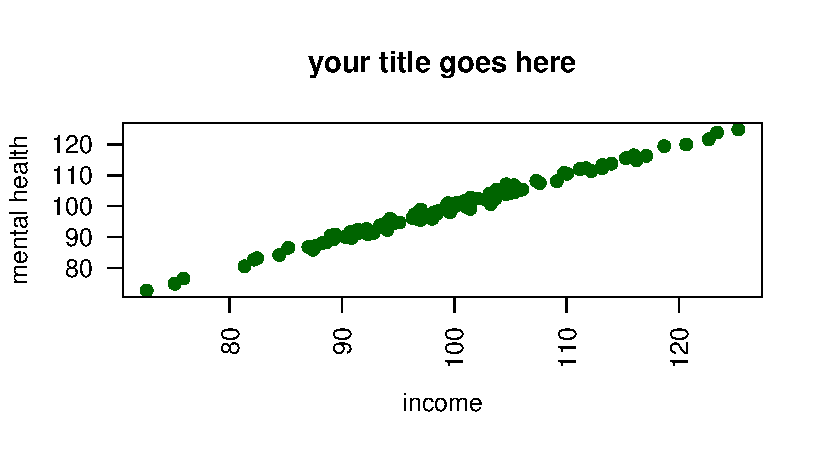
\includegraphics{quick-intro-R_files/figure-pdf/unnamed-chunk-8-1.pdf}

}

\end{figure}

\begin{tcolorbox}[enhanced jigsaw, toptitle=1mm, opacityback=0, colbacktitle=quarto-callout-tip-color!10!white, opacitybacktitle=0.6, arc=.35mm, colframe=quarto-callout-tip-color-frame, coltitle=black, bottomrule=.15mm, leftrule=.75mm, breakable, bottomtitle=1mm, left=2mm, titlerule=0mm, toprule=.15mm, rightrule=.15mm, title=\textcolor{quarto-callout-tip-color}{\faLightbulb}\hspace{0.5em}{Tip}, colback=white]

You often \emph{don't} need to use all of the options.
e.g.~\texttt{plot(mydata\$x,\ mydata\$y)} will work just fine.

\end{tcolorbox}

\begin{tcolorbox}[enhanced jigsaw, toptitle=1mm, opacityback=0, colbacktitle=quarto-callout-tip-color!10!white, opacitybacktitle=0.6, arc=.35mm, colframe=quarto-callout-tip-color-frame, coltitle=black, bottomrule=.15mm, leftrule=.75mm, breakable, bottomtitle=1mm, left=2mm, titlerule=0mm, toprule=.15mm, rightrule=.15mm, title=\textcolor{quarto-callout-tip-color}{\faLightbulb}\hspace{0.5em}{Tip}, colback=white]

When scatterplots have fewer dots than you think they should have, often
due to ``over-printing'', adding some random noise, or ``jittering'' the
dots in the scatterplot may help:
\texttt{plot(jitter(mydata\$y,\ factor\ =\ 5000)\ \textasciitilde{}\ mydata\$x)}.
Experiment with different sizes of \emph{factor}.

\end{tcolorbox}

\hypertarget{analyze-data-descriptive-statistics}{%
\section{Analyze Data: Descriptive
Statistics}\label{analyze-data-descriptive-statistics}}

\begin{Shaded}
\begin{Highlighting}[]
\FunctionTok{summary}\NormalTok{(mydata}\SpecialCharTok{$}\NormalTok{x) }\CommentTok{\# for continuous or factor variables}
\end{Highlighting}
\end{Shaded}

\begin{verbatim}
   Min. 1st Qu.  Median    Mean 3rd Qu.    Max. 
  72.61   92.11   99.53   99.39  104.85  125.28 
\end{verbatim}

\begin{Shaded}
\begin{Highlighting}[]
\FunctionTok{table}\NormalTok{(mydata}\SpecialCharTok{$}\NormalTok{z) }\CommentTok{\# especially suitable for factor variables}
\end{Highlighting}
\end{Shaded}

\begin{verbatim}

 1  2 
73 27 
\end{verbatim}

For another approach to summarizing your data, try:

\begin{Shaded}
\begin{Highlighting}[]
\FunctionTok{library}\NormalTok{(skimr)}

\FunctionTok{skim}\NormalTok{(mydata)}

\FunctionTok{skim}\NormalTok{(mydata}\SpecialCharTok{$}\NormalTok{x)}
\end{Highlighting}
\end{Shaded}




\end{document}
